%% =====================================================================
%% SoundDetect: IEEE conference-format research paper
%% Compile with: pdflatex SoundDetect_IEEE_Paper.tex (run twice)
%% Requires the standard IEEEtran class (bundled with TeX Live / Overleaf).
%% =====================================================================
\documentclass[conference]{IEEEtran}
\IEEEoverridecommandlockouts

\usepackage{cite}
\usepackage{amsmath,amssymb,amsfonts}
\usepackage{algorithm}
\usepackage{algpseudocode}
\usepackage{graphicx}
\usepackage{textcomp}
\usepackage{xcolor}
\usepackage{booktabs}
\usepackage{multirow}
\usepackage{array}
\usepackage{url}
\usepackage{tikz}
\usetikzlibrary{arrows.meta,positioning,shapes.geometric,fit,backgrounds,calc}
\usepackage{pgfplots}
\pgfplotsset{compat=1.17}

\def\BibTeX{{\rm B\kern-.05em{\sc i\kern-.025em b}\kern-.08em
    T\kern-.1667em\lower.7ex\hbox{E}\kern-.125emX}}

\newcommand{\dBFS}{\,dBFS}
\newcommand{\ms}{\,ms}

\begin{document}

\title{SoundDetect: A Local-First Wireless Acoustic Sensor Network for Indoor Sound Event Detection, Classification, and Spatial Mapping}

%% ---------------------------------------------------------------------
%% Replace the placeholder names, departments, and e-mail addresses below.
%% ---------------------------------------------------------------------
\author{
\IEEEauthorblockN{Soham Patil}
\IEEEauthorblockA{\textit{Department of Electronics and}\\
\textit{Telecommunication Engineering}\\
\textit{Name of Institution}\\
City, Country\\
email@institution.edu}
\and
\IEEEauthorblockN{Author Two}
\IEEEauthorblockA{\textit{Department of Electronics and}\\
\textit{Telecommunication Engineering}\\
\textit{Name of Institution}\\
City, Country\\
email@institution.edu}
\and
\IEEEauthorblockN{Author Three}
\IEEEauthorblockA{\textit{Department of Electronics and}\\
\textit{Telecommunication Engineering}\\
\textit{Name of Institution}\\
City, Country\\
email@institution.edu}
\and
\IEEEauthorblockN{Author Four}
\IEEEauthorblockA{\textit{Department of Electronics and}\\
\textit{Telecommunication Engineering}\\
\textit{Name of Institution}\\
City, Country\\
email@institution.edu}
}

\maketitle

%% =====================================================================
\begin{abstract}
A sound-level threshold can report that a room became loud, but it cannot explain what produced the sound or where it happened. This paper presents \emph{SoundDetect}, a local-first Internet-of-Things (IoT) system that detects acoustic events with distributed wireless microphone nodes, classifies them on a local gateway, and places them on an editable floor plan of the monitored room. Two node types share one authenticated HTTPS observation interface: an ESP32 microcontroller with an INMP441 I\textsuperscript{2}S MEMS microphone, and a browser-based smartphone sensor. Each node computes 20\ms{} root-mean-square (RMS) levels in dBFS, applies a per-node threshold that the operator tunes from the dashboard, and uploads only short event clips with a pre-trigger buffer. The gateway validates each clip, groups near-simultaneous observations into one event, classifies it with a general-purpose on-device sound model, estimates a coarse level-weighted position, and evaluates operator-defined composite rules that link ordered sound sequences into named incidents. All processing and storage remain on the local network behind a private certificate authority. We describe the architecture, trigger algorithm, protocol contract, and security model, and report four evaluations: a Monte-Carlo study of the trigger's false-alarm and detection behavior, a 16-event indoor pilot with smartphone sensors, a replay of the pilot clips through the ESP32 trigger logic, and an ingestion latency benchmark. In simulation, a margin of at least 6\,dB above the noise floor produced zero false triggers per hour with the two-frame rule, but the same rule rejected short impulses such as 10\ms{} clicks; in replay, only 8 of 16 field clips satisfied it. The gateway accepted 52\,kB ESP32 uploads with a median ingestion latency of 4.9\ms{}. We discuss the implications for impact detection, calibration, and the planned migration to a Raspberry Pi~5 gateway with MQTT~5 transport.
\end{abstract}

\begin{IEEEkeywords}
Internet of Things, acoustic event detection, wireless acoustic sensor networks, edge computing, ESP32, MEMS microphone, sound classification, smart environments
\end{IEEEkeywords}

%% =====================================================================
\section{Introduction}
\label{sec:intro}

Sound carries information that cameras and motion sensors miss. A knock at the door, a fall in another room, a smoke-alarm chirp, or breaking glass is audible through walls and in darkness, and acoustic sensing is less intrusive than video. These properties have made acoustic monitoring attractive for ambient assisted living, home safety, and building management~\cite{vacher2011,popescu2008,carovia2022}. At the same time, two technical trends have lowered the cost of building such systems. Low-cost microcontrollers with integrated Wi-Fi, such as the ESP32 family~\cite{esp32s3ds}, can read digital MEMS microphones directly over I\textsuperscript{2}S, and pretrained audio classifiers trained on large ontologies such as AudioSet~\cite{gemmeke2017} now run on commodity edge hardware~\cite{hershey2017,kong2020,gong2021}.

Building a dependable indoor system from these parts is still harder than combining a microphone with a model. We identified four problems during the design of the project.

\textbf{P1. Acoustic variation.} Room reverberation, microphone placement, and the gain path of each node change the measured signal level. A threshold expressed in decibels relative to digital full scale (dBFS) is a property of the node, not an acoustic sound pressure level (SPL); equating the two without calibration~\cite{iec61672} leads to inconsistent triggering across nodes.

\textbf{P2. Network delivery.} Consumer and campus Wi-Fi networks disconnect, change addresses, and sometimes isolate clients from one another. Event identity, retry behavior, and clip integrity therefore have to be explicit parts of the protocol.

\textbf{P3. Indoor location.} Satellite positioning is not useful for room-level placement. Events need room-local coordinates tied to a saved floor-plan origin, and the system must not overstate the precision of a position computed from uncalibrated, unsynchronized microphones.

\textbf{P4. Classification.} A general audio model can confuse acoustically similar events, and its label set may not contain the specific actions an operator cares about. Claims about a system's accuracy require labelled recordings from the target rooms and held-out validation.

This paper presents \emph{SoundDetect}, a working prototype that addresses these problems with an event-driven, local-first design. Its contributions are:
\begin{enumerate}
\item an end-to-end architecture in which heterogeneous wireless nodes (an ESP32 + INMP441 microcontroller node and a browser-based smartphone node) share one authenticated observation API, while all classification and storage remain on a local gateway;
\item a node-side trigger based on DC-removed 20\ms{} RMS frames, an operator-tuned per-node dBFS threshold, a minimum-duration rule, a pre-trigger ring buffer, and a cooldown, together with an analysis of its memory and bandwidth cost on the ESP32;
\item a gateway that validates clips, fuses near-simultaneous observations into events, reports an explicitly approximate level-weighted position, and evaluates \emph{composite event rules} that link ordered sound labels into named incidents;
\item a security model built on a private certificate authority whose leaf certificate is re-issued automatically when the gateway's Wi-Fi address changes, so that paired nodes do not need to be re-provisioned; and
\item an evaluation of the trigger, the ingestion path, and a 16-event indoor pilot, with an honest account of which project targets have and have not yet been measured.
\end{enumerate}

The remainder of the paper is organized as follows. Section~\ref{sec:related} reviews related work. Section~\ref{sec:design} describes the system design, and Section~\ref{sec:impl} its implementation. Section~\ref{sec:eval} reports the evaluation, Section~\ref{sec:discussion} discusses the findings and limitations, and Section~\ref{sec:conclusion} concludes.

%% =====================================================================
\section{Related Work}
\label{sec:related}

\subsection{Sound Event Detection and Classification}
Sound event detection (SED) identifies which sound events occur in an audio signal and when~\cite{mesaros2021,stowell2015}. Supervised SED and environmental sound classification were advanced by public datasets such as ESC-50~\cite{piczak2015} and UrbanSound8K~\cite{salamon2014}, and by the much larger weakly labelled AudioSet corpus with an ontology of more than 600 classes~\cite{gemmeke2017}. Convolutional networks trained on log-mel spectrograms became the standard approach~\cite{hershey2017,salamon2017}; convolutional recurrent networks added temporal context for polyphonic detection~\cite{cakir2017}. Pretrained audio neural networks (PANNs)~\cite{kong2020} and the Audio Spectrogram Transformer (AST)~\cite{gong2021} provide strong general-purpose embeddings that can be fine-tuned for a target domain. VGGish-style and YAMNet models derived from this line of work are widely used as baselines on embedded Linux devices. SoundDetect does not propose a new classifier. It treats the classifier as a replaceable gateway component and focuses on the sensing, transport, and event-management layers that surround it.

\subsection{Wireless Acoustic Sensor Networks}
Wireless acoustic sensor networks (WASNs) distribute microphones over an area and combine their observations~\cite{bertrand2011}. Outdoor deployments such as SONYC~\cite{bello2019} monitor urban noise at city scale, and low-cost WASN designs for noise nuisance monitoring have been reported for over a decade~\cite{segura2015}. Indoors, WASNs have been studied for ambient assisted living, where audio can reveal activities of daily living and distress situations~\cite{vacher2011}; acoustic fall detection is a recurring application~\cite{popescu2008}. A recurring design question is where computation should take place: on the node, on a nearby gateway, or in the cloud~\cite{shi2016}. Edge processing reduces bandwidth and keeps raw audio private, but it constrains model size, particularly on microcontrollers~\cite{warden2019}.

\subsection{Closest System Precedents}
Three recent peer-reviewed systems are closest to SoundDetect; Table~\ref{tab:related} compares them.

Saradopoulos~\textit{et~al.}~\cite{saradopoulos2025} built a distributed smart-city audio surveillance system in which ESP32-based microphone nodes send compressed audio over MQTT to Raspberry Pi~5 devices that run an AudioSet-trained transformer. The classified labels are stored as events and organized into graph representations so that hazardous incidents can be queried hierarchically over rolling time windows. This is the nearest end-to-end precedent for wireless capture with gateway inference, and its idea of reasoning over sequences of labels motivated our composite rules. It targets outdoor critical incidents and does not provide an indoor floor plan or per-room configuration.

Segura-Garcia~\textit{et~al.}~\cite{seguragarcia2024} developed a 5G-IoT system for raw audio collection using the same INMP441 microphone and ESP32-S3 microcontroller pair that we use, with convolutional networks that classify up to 41 bird species. It validates the microphone and MCU combination for field audio capture, but it addresses species recognition rather than household events or room localization.

Caro-Via~\textit{et~al.}~\cite{carovia2022} designed an edge-computing meshed WASN for indoor sound monitoring. Each node combines a Raspberry Pi~4B with a USB microphone, nodes form a Wi-Fi mesh, and a Raspberry Pi~4B acts as the gateway; the work also studies sensor placement against acoustic coverage criteria. It is a direct precedent for indoor deployment and sound mapping, but its nodes are single-board computers and its focus is on acoustic levels rather than labelled events.

\begin{table*}[!t]
\centering
\caption{Comparison of SoundDetect with the closest prior systems.}
\label{tab:related}
\renewcommand{\arraystretch}{1.15}
\setlength{\tabcolsep}{4pt}
\begin{tabular}{@{}>{\raggedright\arraybackslash}p{2.6cm}>{\raggedright\arraybackslash}p{3.1cm}>{\raggedright\arraybackslash}p{2.6cm}>{\raggedright\arraybackslash}p{2.7cm}>{\raggedright\arraybackslash}p{1.9cm}>{\raggedright\arraybackslash}p{3.6cm}@{}}
\toprule
\textbf{System} & \textbf{Sensor node} & \textbf{Transport} & \textbf{Inference location} & \textbf{Setting} & \textbf{Spatial / event model} \\
\midrule
Saradopoulos \textit{et al.} 2025~\cite{saradopoulos2025} & ESP32 + I\textsuperscript{2}S MEMS mic & Wi-Fi, MQTT (compressed audio) & Raspberry Pi 5, AST transformer & Outdoor, smart city & Event graph over rolling windows; no indoor map \\
Segura-Garcia \textit{et al.} 2024~\cite{seguragarcia2024} & ESP32-S3 + INMP441 & 5G-IoT & Edge CNN & Outdoor, ecology & Species labels; no localization \\
Caro-Via \textit{et al.} 2022~\cite{carovia2022} & Raspberry Pi 4B + USB mic & Wi-Fi mesh & On node (SBC) & Indoor & Acoustic levels, sound map \\
\textbf{SoundDetect (this work)} & ESP32/ESP32-S3 + INMP441; smartphone browser & Wi-Fi, HTTPS with private CA & Local gateway, on-device sound model & Indoor rooms & Room coordinates, furniture map, composite rules \\
\bottomrule
\end{tabular}
\end{table*}

The selected studies cover the layers of an indoor acoustic event system separately. SoundDetect combines microcontroller and smartphone nodes, local gateway inference, room-local coordinates, playable event clips, and rule-based incident correlation in one system. Cross-room validation of the classifier remains open and is part of our future work.

%% =====================================================================
\section{System Design}
\label{sec:design}

\subsection{Objectives and Acceptance Targets}
The project was specified with four objectives: (i) \emph{capture} 16\,kHz mono audio from an INMP441 through ESP32 I\textsuperscript{2}S with a stable sample format and node identity; (ii) \emph{trigger and report} using 20\ms{} RMS windows with a per-node dBFS threshold and attach time, room coordinates, and level metadata; (iii) \emph{classify} on the gateway and return a top label, a confidence, and an unknown result below a configured floor; and (iv) \emph{present and configure}, i.e., show the event pin, clip, metadata, and node status in a browser and deliver configuration changes back to the node. The design review fixed three proposed acceptance targets: macro-F1 $\geq 0.80$ on labelled test clips, at most 3 false triggers per node-hour, and a 95th-percentile (P95) event-to-UI latency of at most 3\,s on the local network. These are targets, not results; Section~\ref{sec:eval} reports which of them can already be assessed.

\subsection{Architecture Overview}
Fig.~\ref{fig:arch} shows the architecture. It has three execution boundaries. \emph{Sensor nodes} capture audio, apply the trigger, and send event clips with metadata over Wi-Fi. The \emph{gateway} hosts the HTTPS API, validates and stores clips, runs the classifier, maintains the room model, and evaluates composite rules. The \emph{UI client} is a browser that draws the room map, edits configuration, and plays clips; it performs no audio analysis. The system is local-first: the gateway performs inference and serves the dashboard, and no internet connection is needed during operation (the ESP32 uses NTP only to obtain UTC time for certificate validation).

\begin{figure}[!t]
\centering
\resizebox{\columnwidth}{!}{%
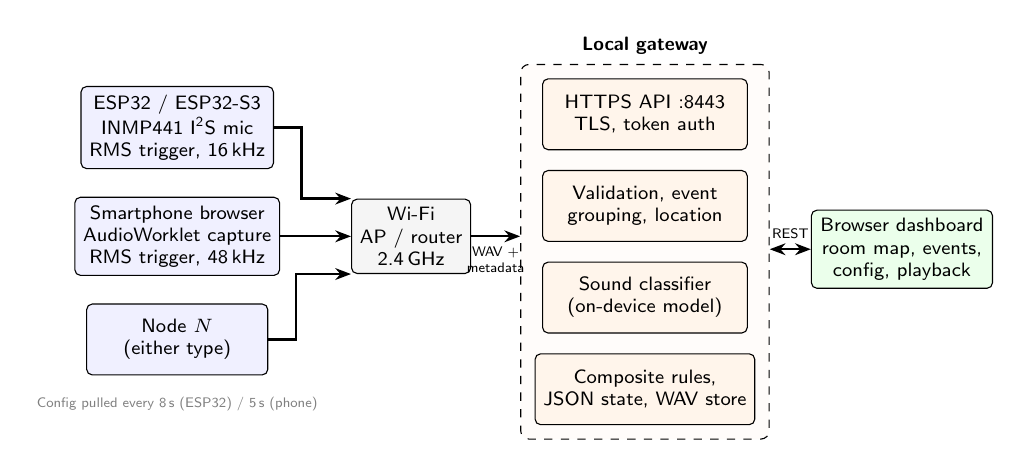
\begin{tikzpicture}[
  font=\sffamily\scriptsize,
  box/.style={draw, rounded corners=2pt, align=center, minimum height=0.9cm, inner sep=3pt, fill=white},
  node/.style={box, fill=blue!6, minimum width=2.3cm},
  gw/.style={box, fill=orange!8, minimum width=2.6cm},
  ui/.style={box, fill=green!8, minimum width=2.3cm},
  arr/.style={-{Stealth[length=2mm]}, thick},
  darr/.style={{Stealth[length=2mm]}-{Stealth[length=2mm]}, thick}
]
\node[node] (esp) {ESP32 / ESP32-S3\\INMP441 I\textsuperscript{2}S mic\\RMS trigger, 16\,kHz};
\node[node, below=0.35cm of esp] (phone) {Smartphone browser\\AudioWorklet capture\\RMS trigger, 48\,kHz};
\node[node, below=0.35cm of phone] (more) {Node $N$\\(either type)};
\node[box, right=0.9cm of phone, minimum width=1.4cm, fill=gray!8] (ap) {Wi-Fi\\AP / router\\2.4\,GHz};

\node[gw, right=0.9cm of ap, yshift=1.55cm] (api) {HTTPS API :8443\\TLS, token auth};
\node[gw, below=0.25cm of api] (store) {Validation, event\\grouping, location};
\node[gw, below=0.25cm of store] (cls) {Sound classifier\\(on-device model)};
\node[gw, below=0.25cm of cls] (rules) {Composite rules,\\JSON state, WAV store};
\begin{scope}[on background layer]
\node[draw, dashed, rounded corners=3pt, fit=(api)(rules), inner sep=5pt, fill=orange!2, label={[font=\sffamily\scriptsize\bfseries]above:Local gateway}] (gwbox) {};
\end{scope}
\node[ui, right=0.8cm of store, yshift=-0.55cm] (dash) {Browser dashboard\\room map, events,\\config, playback};

\draw[arr] (esp.east) -- ++(0.35,0) |- (ap.north west);
\draw[arr] (phone) -- (ap);
\draw[arr] (more.east) -- ++(0.35,0) |- (ap.south west);
\draw[arr] (ap.east) -- node[below, font=\sffamily\tiny, align=center]{WAV +\\metadata} (gwbox.west |- ap.east);
\draw[darr] (gwbox.east |- dash.west) -- node[above, font=\sffamily\tiny]{REST} (dash.west);
\node[below=0.15cm of more, align=center, font=\sffamily\tiny, text=gray] {Config pulled every 8\,s (ESP32) / 5\,s (phone)};
\end{tikzpicture}}
\caption{SoundDetect architecture. Heterogeneous nodes trigger locally and upload short clips over HTTPS; classification, storage, and rule evaluation run only on the local gateway. The browser is a pure presentation client.}
\label{fig:arch}
\end{figure}

\subsection{Sensor Nodes}
\subsubsection{ESP32 + INMP441 node}
The INMP441 is an omnidirectional bottom-port MEMS microphone with a 24-bit I\textsuperscript{2}S output~\cite{inmp441}. The ESP32 acts as I\textsuperscript{2}S master in receive-only mode at 16\,kHz with 32-bit slots and the microphone's L/R pin tied to ground to select the left channel. Because the INMP441 left-aligns its 24-bit sample in the 32-bit slot, the firmware keeps the 16 most significant bits, $x[n] = \lfloor s_{32}[n] / 2^{16} \rfloor$, which yields signed PCM16 for transport. Two board profiles are provided: a classic ESP32 DevKit (BCLK, WS, and data on GPIO 26, 25, and 33) and an ESP32-S3 DevKitC-1 (GPIO 4, 5, and 6). Two FreeRTOS tasks pinned to core~0 handle clock synchronization and configuration polling, while the Arduino loop on the other core reads I\textsuperscript{2}S frames and runs the trigger.

\subsubsection{Smartphone browser node}
Any modern smartphone can join as a node by opening a pairing link. The sensor page requests microphone access with echo cancellation, noise suppression, and automatic gain control disabled, so that the browser does not alter levels between frames. An AudioWorklet delivers blocks of at least 4096 samples (about 85\ms{} at the 48\,kHz rate typical of phones). The page applies the same threshold logic at block granularity, keeps about 0.55\,s of pre-trigger audio, records a clip of about 3.2\,s, applies a 2.1\,s cooldown, and queues up to ten clips with a 4\,s retry interval when the gateway is unreachable. This node type makes it possible to deploy and test the full pipeline before the microcontroller hardware is assembled.

\subsection{Trigger Algorithm}
\label{sec:trigger}
Continuous streaming of 16\,kHz PCM16 audio costs 32\,kB/s, or about 115\,MB per node-hour, and would send every second of a private space off the node. SoundDetect therefore uses an event-driven trigger on the node (Algorithm~\ref{alg:trigger}). For frame $k$ of $M=320$ samples (20\ms{} at 16\,kHz), the node removes the frame mean and computes
\begin{equation}
L_k = 20 \log_{10}\!\left(\frac{1}{32768}\sqrt{\frac{1}{M}\sum_{n=0}^{M-1}\left(x_k[n]-\bar{x}_k\right)^2}\right)\ \text{dBFS},
\label{eq:dbfs}
\end{equation}
with $L_k = -120$\dBFS{} when the RMS is below one least-significant bit. Mean removal suppresses the DC offset present in many MEMS front ends, which would otherwise raise the apparent level. A clip starts when $L_k \geq \theta$ for $N=2$ consecutive frames (40\ms) and the node is not in cooldown, where $\theta$ is the node's threshold. The clip contains the pre-trigger ring buffer (up to 200\ms), the trigger frame, and 1\,s of post-trigger audio, i.e., about 1.22\,s in total. After capture the node enters a 1.8\,s cooldown and uploads the clip. The threshold defaults to $-28$\dBFS{} and is clamped by the gateway to $[-60, -8]$\dBFS.

\begin{algorithm}[!t]
\caption{Node-side event trigger (ESP32 firmware)}
\label{alg:trigger}
\begin{algorithmic}[1]
\Require threshold $\theta$, min.\ frames $N$, cooldown $T_c$, post-roll $P$
\State $h \gets 0$; $\textit{rec} \gets \textbf{false}$; $t_{cd} \gets 0$
\Loop
  \State read frame $x_k$ ($M=320$ samples) from I\textsuperscript{2}S DMA
  \State compute $L_k$ by \eqref{eq:dbfs}
  \If{\textit{rec}}
     \State append $x_k$ to clip; $L_{\max} \gets \max(L_{\max}, L_k)$
     \If{clip length $\geq$ pre-roll $+ M + P$}
        \State $\textit{rec} \gets \textbf{false}$; $t_{cd} \gets \textit{now} + T_c$
        \State \Call{Upload}{clip, $L_{\max}$, UTC time}
     \EndIf
     \State \textbf{continue}
  \EndIf
  \State $h \gets h+1$ \textbf{if} $L_k \geq \theta$ \textbf{else} $0$
  \If{$h \geq N$ \textbf{and} $\textit{now} \geq t_{cd}$}
     \State clip $\gets$ ring buffer $\Vert\ x_k$; $L_{\max} \gets L_k$; $\textit{rec} \gets \textbf{true}$; $h \gets 0$
  \Else
     \State push $x_k$ into pre-trigger ring buffer (200\ms)
  \EndIf
\EndLoop
\end{algorithmic}
\end{algorithm}

Fig.~\ref{fig:timeline} shows the resulting timing of one capture on the ESP32 node.

\begin{figure}[!t]
\centering
\resizebox{\columnwidth}{!}{%
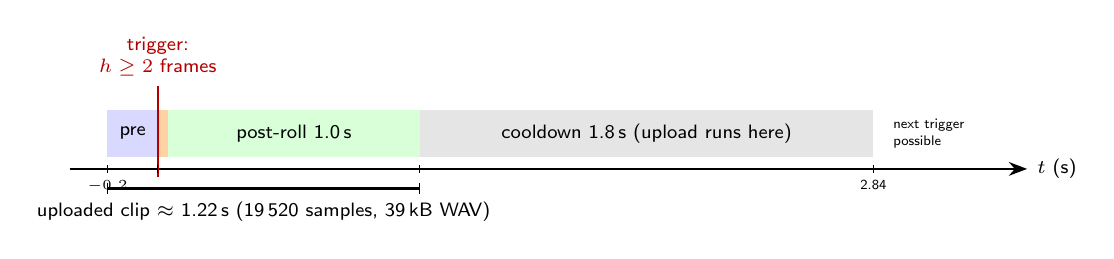
\begin{tikzpicture}[font=\sffamily\scriptsize, x=3.2cm, y=1cm]
\draw[-{Stealth}, thick] (-0.35,0) -- (3.45,0) node[right]{$t$ (s)};
\fill[blue!15] (-0.2,0.15) rectangle (0,0.75);
\fill[orange!35] (0,0.15) rectangle (0.04,0.75);
\fill[green!15] (0.04,0.15) rectangle (1.04,0.75);
\fill[gray!20] (1.04,0.15) rectangle (2.84,0.75);
\node at (-0.1,0.45) {pre};
\node at (0.54,0.45) {post-roll 1.0\,s};
\node at (1.94,0.45) {cooldown 1.8\,s (upload runs here)};
\draw[red!70!black, thick] (0,-0.1) -- (0,1.05) node[above, align=center]{trigger:\\$h \geq 2$ frames};
\draw[decorate, thick] (-0.2,-0.25) -- (1.04,-0.25);
\draw (-0.2,-0.18) -- (-0.2,-0.32); \draw (1.04,-0.18) -- (1.04,-0.32);
\node[below] at (0.42,-0.3) {uploaded clip $\approx$ 1.22\,s (19\,520 samples, 39\,kB WAV)};
\foreach \x/\l in {-0.2/-0.2, 0/0, 1.04/1.04, 2.84/2.84} \draw (\x,0.05) -- (\x,-0.05);
\node[below, font=\sffamily\tiny] at (-0.2,-0.02) {$-0.2$};
\node[below, font=\sffamily\tiny] at (2.84,-0.02) {2.84};
\node[right, align=left, font=\sffamily\tiny] at (2.88,0.45) {next trigger\\possible};
\end{tikzpicture}}
\caption{Timing of one ESP32 capture. The 200\,ms pre-trigger ring buffer, the 40\,ms of trigger frames, and 1\,s of post-roll form the uploaded clip; the node then ignores new triggers for 1.8\,s.}
\label{fig:timeline}
\end{figure}

The minimum-duration rule and the cooldown are the main defences against false triggers from isolated noisy frames and against bursts of uploads from one long event. Section~\ref{sec:eval} shows that the minimum-duration rule also has a cost: it suppresses very short impulsive sounds.

\subsection{Transport, Identity, and Configuration}
Both node types use the same two endpoints over HTTPS on port 8443. A node polls \texttt{GET /api/sensor-config} (every 8\,s on the ESP32, every 5\,s on the phone) to fetch its name and threshold; the poll also refreshes the node's last-seen time and active flag shown in the dashboard. After a trigger, the node sends \texttt{POST /api/observations} with a JSON body containing the sensor identifier, the UTC capture time, the clip's peak level, its duration and sample rate, a firmware identifier, and the WAV file in Base64. The gateway answers \texttt{202 Accepted} with the event and observation identifiers as soon as the clip is stored; classification runs asynchronously. Pulling configuration rather than pushing it means a node needs no listening socket, which suits nodes behind client-isolating Wi-Fi and phones that cannot accept inbound connections. Table~\ref{tab:record} lists the fields that the gateway keeps for each observation; node-supplied values are clamped to physical ranges before storage.

\begin{table}[!t]
\centering
\caption{Observation record stored by the gateway.}
\label{tab:record}
\renewcommand{\arraystretch}{1.08}
\footnotesize
\setlength{\tabcolsep}{4pt}
\begin{tabular}{@{}l l p{3.55cm}@{}}
\toprule
\textbf{Field} & \textbf{Source} & \textbf{Meaning / validation} \\
\midrule
\texttt{id}, \texttt{file} & gateway & Random identifier; WAV file name \\
\texttt{sensorId}, \texttt{sensorName} & token lookup & Authenticated node identity \\
\texttt{sensorPosition} & room model & Node $(x, y)$ in metres from origin \\
\texttt{capturedAt} & node & UTC; replaced if $>300$\,s from gateway clock \\
\texttt{receivedAt} & gateway & UTC receive time \\
\texttt{peakDbfs} & node & Peak frame level, clamped to $[-120, 0]$ \\
\texttt{duration} & WAV header & 0.2--10\,s, from frame count \\
\texttt{sampleRate} & WAV header & 8--96\,kHz \\
\texttt{firmware} & node & e.g., \texttt{esp32-inmp441-v1} \\
\texttt{label}, \texttt{confidence} & classifier & Top label; ``Analyzing\ldots'' until done \\
\texttt{candidates} & classifier & Top-5 labels with raw identifiers \\
\bottomrule
\end{tabular}
\end{table}

\subsection{Gateway Processing}
\subsubsection{Validation}
The gateway authenticates every upload with the node's token and rejects malformed input before it touches storage: the request body is limited to 9\,MB and the decoded audio to 2\,MB; the WAV file must be uncompressed mono 16-bit PCM with a duration between 0.2 and 10\,s and a sample rate between 8 and 96\,kHz. The capture time reported by the node is accepted only if it lies within 300\,s of the gateway clock; otherwise the gateway substitutes its own receive time. This prevents a node with an unsynchronized clock (for example, an ESP32 before its first NTP response) from placing events in 1970.

\subsubsection{Event grouping}
One physical sound may trigger several nodes. The gateway therefore attaches an incoming observation to an existing event if that event's timestamp lies within $\Delta = 2.5$\,s of the observation's capture time, searching the 30 most recent events; otherwise it creates a new event. The event's label and confidence are taken from its most confident classified observation.

\subsubsection{Coarse location}
If one node reports an event, the gateway places the event at that node's position and labels the result ``near reporting sensor; source location unknown.'' If $K \geq 2$ distinct nodes report it, the gateway computes a level-weighted centroid of the node positions $\mathbf{p}_i$:
\begin{equation}
\hat{\mathbf{p}} = \frac{\sum_{i=1}^{K} w_i\, \mathbf{p}_i}{\sum_{i=1}^{K} w_i}, \qquad w_i = \max\!\left(10^{-3},\ 10^{L_i/20}\right),
\label{eq:centroid}
\end{equation}
where $L_i$ is the peak level reported by node $i$. The weight is the linear amplitude, so a node 6\,dB louder receives twice the weight. This estimator is deliberately simple. Because the nodes are neither calibrated nor sample-synchronized, time-difference-of-arrival localization is not possible, and the dashboard labels the result as an approximate estimate from uncalibrated microphones.

\subsubsection{Classification}
Each stored clip is classified in a separate worker thread. The current gateway uses the built-in general sound classifier of Apple's Sound Analysis framework~\cite{applesa}, which recognizes about 300 everyday sound categories. A compiled helper analyses the WAV file in overlapping windows, keeps for each category the maximum confidence observed across windows, and returns the five highest. The gateway maps a few raw identifiers to operator-friendly labels (speech and conversation to \emph{Talking}, clap to \emph{Clapping}, and thump, thud, or crash to \emph{Impact / possible fall}). The wording ``possible fall'' is intentional: an impact sound cannot prove that a person fell. If the classifier is unavailable, clips are stored and shown as unclassified; if analysis fails or times out after 35\,s, the observation is marked ``analysis failed.'' Because the classifier is a separate executable behind a small interface (file in, ranked labels out), it can be replaced by another model without changes to the node protocol.

\subsection{Composite Event Rules}
Many situations of interest are sequences of sounds rather than single sounds. Inspired by the label-graph reasoning of~\cite{saradopoulos2025}, SoundDetect lets the operator define a rule
\begin{equation}
r = (\textit{name},\ a,\ b,\ W,\ \sigma),
\end{equation}
where $a$ and $b$ are case-insensitive label fragments, $W \in [5, 600]$\,s is a time window, and $\sigma \in \{\textit{any\_sensor}, \textit{same\_sensor}\}$ is a scope. Let $\ell(e)$, $t(e)$, and $S(e)$ denote the label, timestamp, and set of reporting nodes of a classified event $e$, and let $t_r$ be the time the rule was created or last edited. A pair of events $(e_1, e_2)$ forms an incident of $r$ if
\begin{equation}
a \sqsubseteq \ell(e_1),\ \ b \sqsubseteq \ell(e_2),\ \ 0 < t(e_2) - t(e_1) \leq W,\ \ t(e_1) \geq t_r,
\end{equation}
where $\sqsubseteq$ denotes substring containment, and, when $\sigma = \textit{same\_sensor}$, $S(e_1) \cap S(e_2) \neq \emptyset$. For each trigger event $e_2$ the gateway links the nearest qualifying $e_1$ and creates at most one incident per rule, which avoids alarm storms when many matching first events precede one second event. Rules are re-evaluated whenever all observations of an event have been classified, so an incident is still found when the second clip finishes classification before the first. For example, a rule named ``Possible break-in'' can link \emph{knock} followed by \emph{door} within 45\,s. These rules correlate recognized labels; they do not establish intent, and the dashboard says so.

\subsection{Room Model and Dashboard}
The room is modelled as a rectangle of configurable width and depth (2--30\,m) with an origin at one corner. New nodes are placed near the four corners, 0.3\,m from the walls, and can be dragged on the map; furniture blocks of seven types (sofa, table, bed, desk, chair, cabinet, plant) can be added to help the operator relate events to the physical space. A room photograph can be uploaded as a visual reference, but the system does not infer geometry from it. The dashboard renders an isometric room map with node markers and event pins, an event log with candidate labels, per-node readings, and playable clips, a compound-event panel, and editors for room, nodes, rules, and furniture. It refreshes its state every 2.5\,s.

\subsection{Security and Privacy Model}
All traffic uses TLS~\cite{rfc8446}. The gateway creates a private certificate authority (RSA-2048, 10-year validity) on first start and issues a leaf certificate (365 days) whose subject-alternative names contain \texttt{localhost}, the loopback address, and the gateway's current LAN address. A monitor thread checks the active Wi-Fi address every 3\,s; when it changes, the gateway re-issues the leaf certificate for the new address with the same CA and reloads it into the live TLS context. Nodes that already trust the CA continue to work without re-pairing. The ESP32 embeds the CA certificate and verifies the server with it; an insecure mode exists only as a compile-time switch for isolated lab debugging and is off by default.

Each node receives a random 192-bit token, and the dashboard is protected by a separate 192-bit administrator key; both are compared in constant time. Because tokens appear in pairing URLs, the gateway suppresses access logging. Static pages are served with a restrictive Content-Security-Policy, \texttt{no-store} caching, \texttt{nosniff}, and \texttt{no-referrer} headers. Audio never leaves the local network: clips are stored only on the gateway, and removing a node from the dashboard revokes its token. Table~\ref{tab:threats} summarizes the threats considered and the corresponding mitigations.

\begin{table}[!t]
\centering
\caption{Threats considered and implemented mitigations.}
\label{tab:threats}
\renewcommand{\arraystretch}{1.08}
\footnotesize
\setlength{\tabcolsep}{4pt}
\begin{tabular}{@{}p{2.7cm}p{5.2cm}@{}}
\toprule
\textbf{Threat} & \textbf{Mitigation} \\
\midrule
Eavesdropping on LAN & TLS on all endpoints; ESP32 verifies the server against the embedded private CA \\
Rogue node injecting clips & Per-node 192-bit token; constant-time comparison; revocation by node removal \\
Unauthorized dashboard access & Separate 192-bit admin key; CSP and no-store headers \\
Malformed or oversized uploads & Size limits; strict WAV format, duration, and rate checks \\
Token leakage via logs & Access logging disabled; \texttt{no-referrer} policy \\
Wrong or forged timestamps & Node time accepted only within $\pm300$\,s of gateway \\
Gateway address change & Automatic leaf re-issue under the same CA \\
\bottomrule
\end{tabular}
\end{table}

%% =====================================================================
\section{Implementation}
\label{sec:impl}

\subsection{Software Stack}
The gateway is a single Python~3 program that uses only the standard library: a threaded HTTP server wrapped in TLS, \texttt{wave} for clip validation, and \texttt{subprocess} for OpenSSL certificate management and the classifier. State (room, furniture, nodes, rules, events, incidents) is held in memory under a re-entrant lock and persisted to a JSON file by atomic write-and-rename after every change; the event and incident lists are capped at the 300 most recent entries. Clips are stored as WAV files named by event and observation identifiers. The classifier is a 37-line Swift program compiled on first start. The dashboard and sensor pages are plain HTML, CSS, and JavaScript with no external dependencies. The ESP32 firmware is an Arduino-framework PlatformIO project of about 430 lines that depends only on ArduinoJson. Table~\ref{tab:api} lists the API.

\begin{table}[!t]
\centering
\caption{Gateway HTTP API (HTTPS, port 8443).}
\label{tab:api}
\renewcommand{\arraystretch}{1.1}
\footnotesize
\setlength{\tabcolsep}{3pt}
\begin{tabular}{@{}l l p{3.3cm}@{}}
\toprule
\textbf{Method} & \textbf{Path} & \textbf{Purpose (auth)} \\
\midrule
GET & \texttt{/api/sensor-config} & Node threshold, name; heartbeat (node token) \\
POST & \texttt{/api/observations} & Upload WAV clip + metadata (node token) \\
GET & \texttt{/api/state} & Room, nodes, events, rules, incidents (admin) \\
GET & \texttt{/api/audio} & Stream a stored clip (admin) \\
POST & \texttt{/api/sensors} & Add a mobile or ESP32 node (admin) \\
PATCH & \texttt{/api/sensors/\{id\}} & Name, threshold, watchlist, position (admin) \\
POST & \texttt{/api/room}, \texttt{/api/photo} & Room geometry, reference photo (admin) \\
POST/PATCH & \texttt{/api/event-rules} & Create, edit, pause composite rules (admin) \\
POST/PATCH & \texttt{/api/furniture} & Place and move furniture (admin) \\
GET & \texttt{/ca.crt} & Download the local CA for node trust \\
\bottomrule
\end{tabular}
\end{table}

\subsection{ESP32 Memory and Payload Budget}
The ESP32 has about 520\,kB of on-chip SRAM, of which a few hundred kilobytes are available to the application once Wi-Fi and TLS are running. Table~\ref{tab:mem} lists the firmware's statically allocated audio buffers and the transient upload buffer. A 1.22\,s clip is 39\,084\,bytes as a WAV file and 52\,221\,bytes as the JSON request body after Base64 encoding (a 33\,\% overhead). Before encoding, the firmware checks that the free heap exceeds the expected body size plus a 70\,kB reserve for the TLS session; if not, it drops the clip and reports why on the serial console instead of failing mid-upload. The WAV header and Base64 encoding are generated on the fly from the sample buffer, so no second copy of the binary WAV is held in memory.

\begin{table}[!t]
\centering
\caption{ESP32 firmware buffers at 16\,kHz.}
\label{tab:mem}
\renewcommand{\arraystretch}{1.1}
\footnotesize
\begin{tabular}{@{}l r l@{}}
\toprule
\textbf{Buffer} & \textbf{Bytes} & \textbf{Allocation} \\
\midrule
Clip buffer (2\,s PCM16) & 64\,000 & static \\
Pre-trigger ring (200\ms) & 6\,400 & static \\
I\textsuperscript{2}S read frame (320 $\times$ 32-bit) & 1\,280 & static \\
PCM16 working frame & 640 & static \\
I\textsuperscript{2}S DMA (8 $\times$ 320 $\times$ 32-bit) & 10\,240 & driver \\
Upload body (1.22\,s clip, Base64 JSON) & $\approx$52\,700 & heap, per upload \\
TLS + free-heap reserve required & 70\,000 & heap guard \\
\bottomrule
\end{tabular}
\end{table}

\subsection{Test Suite}
The repository contains 12 automated unit tests and an end-to-end smoke test. The unit tests cover LAN address selection (preferring the active Wi-Fi address and skipping loopback and link-local addresses), regeneration of pairing links after an address change, live reload of the TLS certificate, rotation of the leaf certificate's subject-alternative names without replacing the trusted CA, persistence of node metadata, creation of both node types, the event-rule API routes, and the composite-rule semantics: ordered matching, out-of-order classification, rejection of wrong order, out-of-window and wrong-scope pairs, same-sensor matching, and pausing a rule. All 12 tests pass in 0.21\,s. The smoke test posts a synthetic WAV file to a running gateway and verifies that the event, observation, and audio are retrievable through the API.

%% =====================================================================
\section{Evaluation}
\label{sec:eval}

We evaluated the parts of the system that can be measured without a labelled dataset: the trigger's false-alarm and detection behavior, the behavior of the ESP32 trigger on real indoor recordings, the gateway's ingestion cost, and a small pilot deployment. We did not measure classification accuracy, battery life, or radio reliability, and we make no claims about them.

\subsection{Trigger False-Alarm Rate (Simulation)}
\label{sec:fa}
We re-implemented Algorithm~\ref{alg:trigger} in Python with the firmware's exact parameters (16\,kHz, 20\ms{} DC-removed RMS frames, 1\,s post-roll, 1.8\,s cooldown). The background was 10 minutes of low-pass-filtered Gaussian noise (a first-order filter with coefficient 0.9, giving a pinkish spectrum) at an RMS level of $-50$\dBFS, with a slow $\pm 3$\,dB sinusoidal gain variation with a 37\,s period to emulate drifting ambient noise. We varied the threshold margin above the nominal noise floor and the minimum number of consecutive frames $N$. Counts were scaled to triggers per hour, so the resolution is 6 per hour.

\begin{table}[!t]
\centering
\caption{Simulated false triggers per hour on noise only ($-50$\dBFS{} mean floor, $\pm3$\,dB drift).}
\label{tab:fa}
\renewcommand{\arraystretch}{1.1}
\begin{tabular}{@{}c c c c@{}}
\toprule
\textbf{Margin $\theta - L_{\text{noise}}$} & $N=1$ & $N=2$ (default) & $N=3$ \\
\midrule
3\,dB & 522 & 330 & 216 \\
6\,dB & 12 & \textbf{0} & 0 \\
9\,dB & 0 & 0 & 0 \\
12\,dB & 0 & 0 & 0 \\
\bottomrule
\end{tabular}
\end{table}

Table~\ref{tab:fa} shows that a 3\,dB margin is unusable: the drifting noise crosses the threshold hundreds of times per hour, and requiring more frames only reduces the rate. With a 6\,dB margin, $N=1$ still produced 12 false triggers per hour, four times the project target, while $N=2$ produced none. At 9\,dB or more, the frame rule no longer matters for this noise model. In this model, the default $N=2$ meets the target of at most 3 false triggers per node-hour once the threshold sits at least 6\,dB above the ambient floor. Real rooms contain non-stationary sounds (speech, appliances, traffic) that this model omits, so these numbers bound the stationary-noise contribution only.

\subsection{Detection Versus Event Level and Duration (Simulation)}
We then inserted synthetic events into 1\,s noise segments ($-50$\dBFS) at a random offset and counted how often the default trigger ($\theta = -28$\dBFS, $N=2$) fired. Each event was white noise with an exponential envelope; four types differed in duration and decay constant $\tau$: a \emph{click} (10\ms, $\tau = 3$\ms), a \emph{knock} (60\ms, $\tau = 20$\ms), a \emph{clap} (150\ms, $\tau = 40$\ms), and a sustained \emph{speech-like} burst (400\ms, $\tau = 1$\,s). The event level is the RMS of its first 20\ms{} relative to $\theta$. Each point in Fig.~\ref{fig:detect} is the fraction of 60 trials that triggered.

\begin{figure}[!t]
\centering
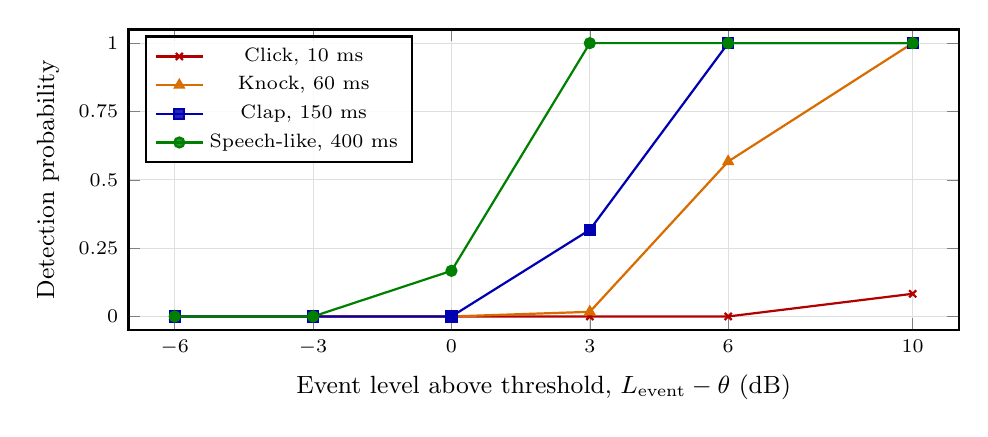
\begin{tikzpicture}
\begin{axis}[
  width=\columnwidth, height=5.4cm,
  xlabel={Event level above threshold, $L_{\text{event}}-\theta$ (dB)},
  ylabel={Detection probability},
  xmin=-7, xmax=11, ymin=-0.05, ymax=1.05,
  xtick={-6,-3,0,3,6,10},
  ytick={0,0.25,0.5,0.75,1},
  grid=major, grid style={gray!25},
  legend style={font=\scriptsize, at={(0.02,0.98)}, anchor=north west, fill=white, fill opacity=0.85, text opacity=1},
  tick label style={font=\scriptsize}, label style={font=\small},
  mark size=1.8pt, thick
]
\addplot[color=red!70!black, mark=x] coordinates {(-6,0) (-3,0) (0,0) (3,0) (6,0) (10,0.083)};
\addlegendentry{Click, 10 ms}
\addplot[color=orange!85!black, mark=triangle*] coordinates {(-6,0) (-3,0) (0,0) (3,0.017) (6,0.567) (10,1.0)};
\addlegendentry{Knock, 60 ms}
\addplot[color=blue!70!black, mark=square*] coordinates {(-6,0) (-3,0) (0,0) (3,0.317) (6,1.0) (10,1.0)};
\addlegendentry{Clap, 150 ms}
\addplot[color=green!50!black, mark=*] coordinates {(-6,0) (-3,0) (0,0.167) (3,1.0) (6,1.0) (10,1.0)};
\addlegendentry{Speech-like, 400 ms}
\end{axis}
\end{tikzpicture}
\caption{Simulated detection probability of the default trigger ($\theta=-28$\dBFS, $N=2$ frames of 20\,ms) for four synthetic event types, 60 trials per point. Short, fast-decaying impulses need far more headroom to be detected, and 10\,ms clicks are almost always rejected.}
\label{fig:detect}
\end{figure}

Sustained sounds were detected reliably from 3\,dB above the threshold. Decaying impulses needed more headroom because the second 20\ms{} frame must also exceed $\theta$: the clap reached full detection at 6\,dB and the knock only at 10\,dB, and the 10\ms{} click was detected in only 8\,\% of trials even at 10\,dB. The two-frame rule therefore behaves as a duration filter. That is useful against isolated electrical or mechanical clicks, but it works against detection of impacts, which are among the most safety-relevant indoor sounds.

\subsection{Indoor Pilot with Smartphone Nodes}
To exercise the full pipeline before the ESP32 hardware was assembled, we ran a pilot in a 6\,m $\times$ 5\,m living-room model with smartphone nodes at the default corner positions. The gateway was a MacBook running the Apple Sound Analysis classifier. During two sessions (1 and 15 October 2026), two phone nodes produced 16 events, each from a single node; the phones recorded at 48\,kHz, giving 3.24\,s clips of 311\,kB. Sounds were produced informally during development testing (talking, clapping, knocking, tapping, and similar actions); no ground-truth annotation was recorded, so the pilot measures system behavior, not accuracy.

\begin{table}[!t]
\centering
\caption{Pilot events: top classifier label, confidence, and peak level reported by the phone node.}
\label{tab:pilot}
\renewcommand{\arraystretch}{1.05}
\footnotesize
\begin{tabular}{@{}l c c c@{}}
\toprule
\textbf{Top label} & \textbf{Events} & \textbf{Confidence} & \textbf{Peak (dBFS)} \\
\midrule
Talking & 8 & 0.505--0.919 (mean 0.789) & $-38.7$ to $-25.2$ \\
Sneeze & 1 & 0.965 & $-17.0$ \\
Knock & 1 & 0.696 & $-24.0$ \\
Slap / smack & 1 & 0.619 & $-16.7$ \\
Tap & 1 & 0.544 & $-18.3$ \\
Clapping & 1 & 0.318 & $-21.4$ \\
Hammer & 1 & 0.298 & $-27.8$ \\
Firecracker & 1 & 0.160 & $-11.4$ \\
Music & 1 & 0.086 & $-26.5$ \\
\midrule
\textbf{All} & \textbf{16} & median 0.716, mean 0.625 & $-38.7$ to $-11.4$ \\
\bottomrule
\end{tabular}
\end{table}

Table~\ref{tab:pilot} summarizes the events. Every clip was received, stored, classified, and shown on the map with a playable recording, and the dashboard displayed the top five candidates for each. Speech dominated, and speech events received consistently high confidence (mean 0.789). The eight non-speech events had a mean confidence of only 0.461, and several were labelled with semantically adjacent categories: the \emph{knock} event listed \emph{door} (0.56) and \emph{hammer} (0.38) as its next candidates, and the \emph{tap} event listed \emph{clapping} and \emph{impact / possible fall}. This illustrates problem P4: a general model often ranks the right family of sounds highly but separates its members poorly. With the proposed confidence floor of 0.5, four of the 16 events (25\,\%) would be reported as unknown, which is the intended behavior for low-certainty impulsive sounds. Peak levels spanned 27\,dB, from quiet speech at $-38.7$\dBFS{} to an impulsive sound at $-11.4$\dBFS, which shows why a fixed, uncalibrated threshold cannot serve every node and every sound. Fig.~\ref{fig:pilot} plots confidence against peak level and shows no simple relation between loudness and classifier certainty: the loudest event (\emph{firecracker}, $-11.4$\dBFS) received one of the lowest confidences, while quiet speech at $-36.1$\dBFS{} received 0.80.

\begin{figure}[!t]
\centering
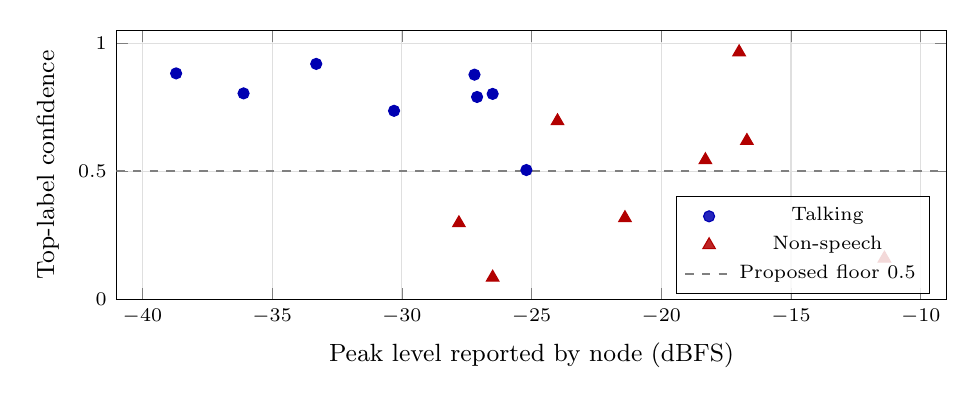
\begin{tikzpicture}
\begin{axis}[
  width=\columnwidth, height=5.0cm,
  xlabel={Peak level reported by node (dBFS)},
  ylabel={Top-label confidence},
  xmin=-41, xmax=-9, ymin=0, ymax=1.05,
  grid=major, grid style={gray!25},
  legend style={font=\scriptsize, at={(0.98,0.02)}, anchor=south east, fill=white, fill opacity=0.85, text opacity=1},
  tick label style={font=\scriptsize}, label style={font=\small},
  mark size=2pt
]
\addplot[only marks, mark=*, color=blue!70!black] coordinates {
(-25.2,0.505) (-36.1,0.804) (-30.3,0.736) (-33.3,0.919) (-38.7,0.882) (-27.1,0.79) (-26.5,0.802) (-27.2,0.877)};
\addlegendentry{Talking}
\addplot[only marks, mark=triangle*, color=red!70!black, mark size=2.6pt] coordinates {
(-21.4,0.318) (-24.0,0.696) (-26.5,0.086) (-18.3,0.544) (-16.7,0.619) (-27.8,0.298) (-17.0,0.965) (-11.4,0.160)};
\addlegendentry{Non-speech}
\addplot[dashed, gray, thick, domain=-41:-9] {0.5};
\addlegendentry{Proposed floor 0.5}
\end{axis}
\end{tikzpicture}
\caption{Pilot events: classifier confidence versus the peak level reported by the phone node. Points below the dashed line would be reported as unknown under the proposed confidence floor.}
\label{fig:pilot}
\end{figure}

\subsection{Replaying Pilot Clips Through the ESP32 Trigger}
The phone node evaluates levels over blocks of about 85\ms, whereas the ESP32 uses 20\ms{} frames. To estimate how the microcontroller node would have treated the same sounds, we decimated each pilot clip from 48 to 16\,kHz (a three-tap moving average followed by 3:1 decimation, which is adequate for level estimation but not for listening) and ran the firmware trigger with $\theta = -28$\dBFS{} and $N=2$. Each pilot clip contains the phone's 0.55\,s pre-trigger audio and the whole event.

Only 8 of the 16 clips triggered. Four of the eight that did not were speech: in three, the loudest 20\ms{} frame stayed below $-28$\dBFS{} (they had been captured while the phone's threshold was set lower), and in the fourth only a single frame, at $-27.7$\dBFS, crossed it. The more instructive failures are four loud impulsive events, labelled \emph{firecracker}, \emph{clapping}, \emph{hammer}, and \emph{tap}, whose loudest 20\ms{} frames reached $-15.0$, $-15.8$, $-20.7$, and $-14.0$\dBFS, between 7 and 14\,dB above the threshold, yet which never had two consecutive frames above it. The \emph{firecracker} clip, for example, had a single frame above threshold. This field result agrees with Fig.~\ref{fig:detect}: on the ESP32, the two-frame rule would miss loud but short impacts that the phone's longer analysis blocks detected. Possible remedies, which we plan to evaluate on labelled data, are (i) a dual-path trigger that fires on either $N=2$ frames above $\theta$ or one frame above $\theta + \delta$ for a margin $\delta$ of 6--10\,dB, (ii) a peak-sample or crest-factor criterion alongside RMS, and (iii) an adaptive threshold $\theta = \hat{L}_{\text{noise}} + m$ that tracks a running noise-floor estimate.

\subsection{Gateway Ingestion Latency}
We measured the cost of the ingestion path in isolation. The unmodified gateway code ran on a 4-core ARM64 Linux virtual machine with Python~3.10 and the classifier replaced by a stub, so that classification time was excluded. A client on the same host posted 120 observations of each clip type over HTTPS (one new TLS connection per request, as the ESP32 does), discarding the first ten as warm-up.

\begin{table}[!t]
\centering
\caption{Gateway ingestion latency over loopback HTTPS, classifier excluded ($n = 110$ per row).}
\label{tab:latency}
\renewcommand{\arraystretch}{1.1}
\footnotesize
\begin{tabular}{@{}l r r r r@{}}
\toprule
\textbf{Clip} & \textbf{Body} & \textbf{Median} & \textbf{P95} & \textbf{Max} \\
\midrule
ESP32, 16\,kHz, 1.22\,s & 52.2\,kB & 4.9\ms & 5.7\ms & 6.5\ms \\
Phone, 48\,kHz, 3.24\,s & 415.3\,kB & 5.7\ms & 6.4\ms & 6.8\ms \\
State query & -- & 1.2\ms & -- & -- \\
\bottomrule
\end{tabular}
\end{table}

Table~\ref{tab:latency} shows that authentication, Base64 decoding, WAV validation, storage, event grouping, location estimation, and the atomic state write together take about 5\ms{} per clip, and that an eightfold larger phone clip adds less than 1\ms. Ingestion is therefore not the bottleneck. These figures exclude Wi-Fi transfer and classification, and the machine differs from the pilot gateway.

\subsection{End-to-End Latency Budget}
Because the full path has not yet been timed with hardware, we decompose it to see whether the 3\,s P95 target is plausible. From the trigger frame, the ESP32 records 1.0\,s of post-roll before it uploads. A 52\,kB body over 2.4\,GHz Wi-Fi adds a TLS handshake and transfer that we expect to take on the order of a few hundred milliseconds. Ingestion adds about 5\ms. Classification time on the gateway is not yet measured. Finally, the dashboard polls every 2.5\,s, so a completed result waits on average 1.25\,s and at worst 2.5\,s before it is drawn. The polling interval alone can consume most of the 3\,s budget at the 95th percentile. The planned WebSocket push (Section~\ref{sec:future}) removes this term and leaves the post-roll and classification as the dominant components.

\subsection{Bandwidth}
An ESP32 node sends 52.2\,kB per event plus a configuration poll every 8\,s. At ten events per hour, the event traffic is about 0.5\,MB per node-hour, roughly 200 times less than continuous 16\,kHz streaming (115\,MB). Phone nodes send 415\,kB per event because they record at 48\,kHz for 3.2\,s; resampling to 16\,kHz in the browser before upload would cut this by a factor of three without affecting the 16\,kHz classifiers we plan to use.

%% =====================================================================
\section{Discussion}
\label{sec:discussion}

\subsection{Lessons from the Prototype}
\emph{The trigger is a classifier in its own right.} Every downstream stage sees only the sounds that the node chooses to send. Our simulation and replay show that the minimum-duration rule, introduced to limit false triggers, is the main reason that short impacts are missed. Trigger parameters should therefore be tuned jointly with the classifier on the same labelled data, and the false-trigger target and the impact recall should be reported together.

\emph{Levels are node-relative.} The 27\,dB spread of pilot peaks and the difference between 20\ms{} and 85\ms{} analysis windows show that the same sound produces different numbers on different nodes. SoundDetect therefore labels every level as dBFS and never presents it as dB SPL. Displaying calibrated SPL would require a per-node calibration against a reference source and a sound level meter~\cite{iec61672}.

\emph{Honest spatial output.} The level-weighted centroid in~\eqref{eq:centroid} is only a coarse indication. Directivity, occlusion by furniture, and reverberation all affect the received level, and single-node events carry no source location at all. The interface states this rather than drawing a precise-looking pin.

\emph{Local-first operation is practical.} A private CA with automatic leaf rotation let nodes survive Wi-Fi address changes during the pilot without re-pairing. Some campus networks, however, block client-to-client traffic, and no software change can bypass that; in such networks, the gateway and nodes need a personal hotspot or a dedicated access point.

\subsection{Design Evolution: Planned Versus Implemented}
The project's design review specified a Raspberry Pi~5 gateway with a Mosquitto MQTT~5 broker over TLS, a FastAPI service with WebSocket push, a YAMNet-based classifier with a project-specific head, and SQLite storage, with a MacBook used only as the UI client. The working prototype reached the same functional boundaries with fewer components. Table~\ref{tab:evolution} compares the two. The node firmware and API are already compatible with a different gateway host, because nodes see only the HTTPS observation contract.

\begin{table}[!t]
\centering
\caption{Reference design from the project review versus the current prototype.}
\label{tab:evolution}
\renewcommand{\arraystretch}{1.1}
\footnotesize
\begin{tabular}{@{}p{1.55cm}p{3.0cm}p{3.0cm}@{}}
\toprule
\textbf{Aspect} & \textbf{Reference design} & \textbf{Current prototype} \\
\midrule
Gateway & Raspberry Pi 5 & MacBook (macOS) \\
Metadata & MQTT 5, QoS 1, TLS :8883 & HTTPS JSON :8443 \\
Audio & HTTPS PUT by event UUID & Base64 WAV in the same POST \\
Classifier & YAMNet + custom head & Apple Sound Analysis \\
Storage & SQLite + WAV store & JSON state + WAV store \\
UI updates & WebSocket push & 2.5\,s polling \\
Config & Retained MQTT topic & Node polls every 5--8\,s \\
Clip (ESP32) & 250\ms{} pre / 1.5\,s post & 200\ms{} pre / 1.0\,s post \\
Integrity & SHA-256, event UUID & Server-side WAV validation \\
\bottomrule
\end{tabular}
\end{table}

\subsection{Limitations}
\label{sec:limits}
This study has clear limits. The pilot is small (16 events, two sessions, one room) and unlabelled, so no accuracy figure can be reported. The ESP32 node has been implemented but not yet measured on hardware, so its battery life, radio reliability, and timing are not reported. The replay experiment used decimated phone recordings, whose microphone and front-end processing differ from the INMP441. The trigger simulation used a stationary noise model. The latency benchmark excluded Wi-Fi and classification and ran on different hardware from the pilot gateway. Finally, the ESP32 upload is synchronous, so the node can miss a second event while sending a clip, and a failed upload is not retried.

\subsection{Ethical Considerations}
Acoustic monitoring of living spaces raises privacy concerns even when it is event-driven. SoundDetect keeps raw audio on the local network, sends audio only after a trigger, and protects every endpoint with a per-node or administrator secret. Deployments should still inform occupants, place nodes away from spaces where conversation is expected to be private, and set a retention period for stored clips. The labels and composite rules are intended as assistive signals for a human operator; they should not be used as evidence of a person's actions or intent.

%% =====================================================================
\section{Future Work}
\label{sec:future}
The next test gate, defined in the project review, is to assemble one battery-powered ESP32-S3 + INMP441 node, record 100 labelled clips across four sound classes in the target room, integrate the node with the gateway, run reconnection and duplicate-message tests, and report macro-F1, false triggers per node-hour, and P95 event-to-UI latency against the targets of Section~\ref{sec:design}. Beyond that milestone we plan to:
\begin{itemize}
\item move the gateway to a Raspberry Pi~5 and replace the classifier with a 16\,kHz YAMNet or PANNs embedding with a project-specific head, trained and validated on held-out room sessions with an explicit unknown class;
\item add MQTT~5 metadata transport with QoS~1~\cite{mqtt5}, retained configuration and status topics, and a Last-Will message for offline detection, and make clip uploads idempotent by event UUID and SHA-256 digest so that at-least-once redelivery cannot create duplicate events;
\item replace dashboard polling with WebSocket push to remove up to 2.5\,s from the event-to-UI path;
\item evaluate the dual-path and adaptive triggers proposed in Section~\ref{sec:eval} and make the ESP32 upload asynchronous with a small retry queue;
\item calibrate each node against a reference source so that dB SPL can be displayed, and study time synchronization among nodes as a prerequisite for time-difference-of-arrival localization; and
\item store room-local $(x, y, z)$ coordinates and extend the room model beyond a single rectangle.
\end{itemize}

%% =====================================================================
\section{Conclusion}
\label{sec:conclusion}
This paper presented SoundDetect, a local-first wireless acoustic sensor network that detects sound events on ESP32 and smartphone nodes, classifies and stores them on a local gateway, places them on an editable room map, and correlates ordered sounds into named incidents. The design keeps raw audio on the local network, authenticates every node, and survives gateway address changes without re-pairing. Our evaluation showed that ingestion costs only about 5\ms{} per clip and is not a bottleneck, that a threshold at least 6\,dB above the noise floor with a two-frame rule removes false triggers from stationary noise, and that the same two-frame rule rejects short, loud impacts, which half of the pilot clips illustrate when replayed through the ESP32 trigger. These results point to the trigger, not the network or the gateway, as the component that most needs joint tuning with the classifier. The next milestone is a measured, labelled evaluation of the battery-powered ESP32 node against the project's accuracy, false-alarm, and latency targets.

\section*{Acknowledgment}
The authors thank the course instructors and reviewers for their feedback during the project design review.

%% =====================================================================
\begin{thebibliography}{00}

\bibitem{saradopoulos2025}
I. Saradopoulos, I. Potamitis, S. Ntalampiras, I. Rigakis, C. Manifavas, and A. Konstantaras, ``Real-time acoustic detection of critical incidents in smart cities using artificial intelligence and edge networks,'' \textit{Sensors}, vol. 25, no. 8, Art. no. 2597, Apr. 2025, doi: 10.3390/s25082597.

\bibitem{seguragarcia2024}
J. Segura-Garcia, S. Sturley, M. Arevalillo-Herraez, J. M. Alcaraz-Calero, S. Felici-Castell, and E. A. Navarro-Camba, ``5G AI-IoT system for bird species monitoring and song classification,'' \textit{Sensors}, vol. 24, no. 11, Art. no. 3687, Jun. 2024, doi: 10.3390/s24113687.

\bibitem{carovia2022}
S. Caro-Via, E. Vida\~{n}a-Vila, G. J. Ginovart-Panisello, C. Mart\'{i}nez-Suqu\'{i}a, M. Freixes, and R. M. Alsina-Pag\`{e}s, ``Edge-computing meshed wireless acoustic sensor network for indoor sound monitoring,'' \textit{Sensors}, vol. 22, no. 18, Art. no. 7032, Sep. 2022, doi: 10.3390/s22187032.

\bibitem{gemmeke2017}
J. F. Gemmeke \textit{et al.}, ``Audio Set: An ontology and human-labeled dataset for audio events,'' in \textit{Proc. IEEE Int. Conf. Acoust., Speech, Signal Process. (ICASSP)}, 2017, pp. 776--780.

\bibitem{hershey2017}
S. Hershey \textit{et al.}, ``CNN architectures for large-scale audio classification,'' in \textit{Proc. IEEE Int. Conf. Acoust., Speech, Signal Process. (ICASSP)}, 2017, pp. 131--135.

\bibitem{kong2020}
Q. Kong, Y. Cao, T. Iqbal, Y. Wang, W. Wang, and M. D. Plumbley, ``PANNs: Large-scale pretrained audio neural networks for audio pattern recognition,'' \textit{IEEE/ACM Trans. Audio, Speech, Lang. Process.}, vol. 28, pp. 2880--2894, 2020.

\bibitem{gong2021}
Y. Gong, Y.-A. Chung, and J. Glass, ``AST: Audio spectrogram transformer,'' in \textit{Proc. Interspeech}, 2021, pp. 571--575.

\bibitem{mesaros2021}
A. Mesaros, T. Heittola, T. Virtanen, and M. D. Plumbley, ``Sound event detection: A tutorial,'' \textit{IEEE Signal Process. Mag.}, vol. 38, no. 5, pp. 67--83, Sep. 2021.

\bibitem{stowell2015}
D. Stowell, D. Giannoulis, E. Benetos, M. Lagrange, and M. D. Plumbley, ``Detection and classification of acoustic scenes and events,'' \textit{IEEE Trans. Multimedia}, vol. 17, no. 10, pp. 1733--1746, Oct. 2015.

\bibitem{piczak2015}
K. J. Piczak, ``ESC: Dataset for environmental sound classification,'' in \textit{Proc. 23rd ACM Int. Conf. Multimedia}, 2015, pp. 1015--1018.

\bibitem{salamon2014}
J. Salamon, C. Jacoby, and J. P. Bello, ``A dataset and taxonomy for urban sound research,'' in \textit{Proc. 22nd ACM Int. Conf. Multimedia}, 2014, pp. 1041--1044.

\bibitem{salamon2017}
J. Salamon and J. P. Bello, ``Deep convolutional neural networks and data augmentation for environmental sound classification,'' \textit{IEEE Signal Process. Lett.}, vol. 24, no. 3, pp. 279--283, Mar. 2017.

\bibitem{cakir2017}
E. \c{C}ak{\i}r, G. Parascandolo, T. Heittola, H. Huttunen, and T. Virtanen, ``Convolutional recurrent neural networks for polyphonic sound event detection,'' \textit{IEEE/ACM Trans. Audio, Speech, Lang. Process.}, vol. 25, no. 6, pp. 1291--1303, Jun. 2017.

\bibitem{bertrand2011}
A. Bertrand, ``Applications and trends in wireless acoustic sensor networks: A signal processing perspective,'' in \textit{Proc. 18th IEEE Symp. Commun. Veh. Technol. Benelux (SCVT)}, 2011, pp. 1--6.

\bibitem{bello2019}
J. P. Bello \textit{et al.}, ``SONYC: A system for monitoring, analyzing, and mitigating urban noise pollution,'' \textit{Commun. ACM}, vol. 62, no. 2, pp. 68--77, Feb. 2019.

\bibitem{segura2015}
J. Segura-Garcia, S. Felici-Castell, J. J. Perez-Solano, M. Cobos, and J. M. Navarro, ``Low-cost alternatives for urban noise nuisance monitoring using wireless sensor networks,'' \textit{IEEE Sensors J.}, vol. 15, no. 2, pp. 836--844, Feb. 2015.

\bibitem{vacher2011}
M. Vacher, F. Portet, A. Fleury, and N. Noury, ``Development of audio sensing technology for ambient assisted living: Applications and challenges,'' \textit{Int. J. E-Health Med. Commun.}, vol. 2, no. 1, pp. 35--54, 2011.

\bibitem{popescu2008}
M. Popescu, Y. Li, M. Skubic, and M. Rantz, ``An acoustic fall detector system that uses sound height information to reduce the false alarm rate,'' in \textit{Proc. 30th Annu. Int. Conf. IEEE Eng. Med. Biol. Soc. (EMBC)}, 2008, pp. 4628--4631.

\bibitem{shi2016}
W. Shi, J. Cao, Q. Zhang, Y. Li, and L. Xu, ``Edge computing: Vision and challenges,'' \textit{IEEE Internet Things J.}, vol. 3, no. 5, pp. 637--646, Oct. 2016.

\bibitem{warden2019}
P. Warden and D. Situnayake, \textit{TinyML: Machine Learning with TensorFlow Lite on Arduino and Ultra-Low-Power Microcontrollers}. Sebastopol, CA, USA: O'Reilly Media, 2019.

\bibitem{esp32s3ds}
Espressif Systems, ``ESP32-S3 series datasheet,'' Shanghai, China. [Online]. Available: https://www.espressif.com

\bibitem{inmp441}
InvenSense Inc., ``INMP441: Omnidirectional microphone with bottom port and I\textsuperscript{2}S digital output,'' Datasheet DS-INMP441-00.

\bibitem{applesa}
Apple Inc., ``Sound Analysis,'' Apple Developer Documentation. [Online]. Available: https://developer.apple.com/documentation/soundanalysis

\bibitem{mqtt5}
OASIS, ``MQTT version 5.0,'' OASIS Standard, Mar. 2019.

\bibitem{iec61672}
\textit{Electroacoustics---Sound Level Meters---Part 1: Specifications}, IEC Standard 61672-1:2013, 2013.

\bibitem{rfc8446}
E. Rescorla, ``The Transport Layer Security (TLS) protocol version 1.3,'' IETF RFC 8446, Aug. 2018.

\end{thebibliography}

\end{document}
